\newpage

\section{Własności}

\subsection{Fazy krystaliczne siarczku galu}
Struktura pasmowa i przerwa energetyczna to są kluczowe parametry dla półprzewodników chalkogenowych. \textit{Chalkogenki} – nieorganiczne związki chemiczne, w których anionami są chalkogeny, tj. siarczki, selenki i telurki. Przykładowymi chalkogenkami są związki $\mathbf{GaS}$, $\mathbf{Ga_{2}S_{3}}$, $\mathbf{GaSe}$, $\mathbf{Ga_{2}Se_{3}}$, które należą do związków III-VI (III: \textbf{In}, \textbf{Ga} i VI: \textbf{S}, \textbf{Se}, \textbf{Te}) grupy układu okresowego. Materiał  $\mathbf{Ga_{2}S_{3}}$ wyróżnia się wśród związków III-VI, szerokością przerwy energetycznej (materiał szerokoprzerwowy). Różna walencyjność atomów grupy III i VI sprawia, że materiał ten ma różne stechiometrie, różne sieci krystaliczne i wynikające stąd odmienne fazy krystaliczne[2][3]. Najbardziej rozpowszechnionymi spośród siarczków galu są związki: siarczek galu II ($\mathbf{GaS}$) oraz siarczek galu III ($\mathbf{Ga_{2}S_{3}}$) 

$\mathbf{GaS}$ podobnie jak $\mathbf{GaSe}$ krystalizuje w heksagonalnej strukturze warstwowej, przy czym ułożenie warstw jest charakterystyczne dla tak zwanej fazy $\beta$. $\mathbf{GaSe}$ posiada prostą przerwę energetyczną wynoszącą około 2 eV, natomiast materiał $\mathbf{GaS}$ jest półprzewodnikiem o skośnej przerwie energetycznej o wartości 2.53 eV[6].

Zarówno $\mathbf{Ga_{2}S_{3}}$ jak i $\mathbf{Ga_{2}Se_{3}}$ krystalizują w tzw. zdefektowanej strukturze blendy cynkowej, w której 1/3 miejsc kationowych jest pusta (położenie luk jest różne w różnych fazach krystalicznych tych materiałów). Jeżeli chodzi o $\mathbf{Ga_{2}Se_{3}}$ to jest to półprzewodnik z prostą przerwą energetyczną o wartości 2-2.4eV[7].

Widać stąd że wszystkie wymienione wyżej chalkogenki $\mathbf{GaSe}$, $\mathbf{GaS}$, $\mathbf{Ga_{2}Se_{3}}$ mają wartości przerwy energetycznej poniżej 2.55 eV. Dla tego też mogą być rozpatrywane czy brane pod uwagę jako materiały do zastosowań w zakresie widzialnym, a nie do zastosowań w zakresie UV jak $\mathbf{Ga_{2}S_{3}}$[8][9].

Poniżej omówiona zostanie budowa krystaliczna dwóch postaci siarczku galu:
\begin{itemize}
	\item Siarczek galu(II) - $\mathbf{GaS}$
	\item Siarczek galu(III) - $\mathbf{Ga_{2}S_{3}}$
\end{itemize}
%grupa przestrzenna $\mathbf{P\;6_{3}/mmc}$
$\mathbf{GaS}$ tworzy bezbarwne lub żółte kryształki o budowie heksagonalnej. Kryształ siarczku galu $\mathbf{(GaS)}$ należy do rodziny półprzewodników warstwowych III-VI. Krystalizuje się w sześciokątnej strukturze o parametrach sieci $a = 0,3578$ i $c = 1,547$ nm. Każda warstwa w strukturze krystalicznej składa się z dwóch warstw atomów galu i dwóch warstw atomów siarki ułożonych prostopadle do osi $c$ z powtarzającą się jednostką $\mathbf{S-Ga-Ga-S}$ [11][12][13].
\begin{figure}[H]
	\begin{center}
		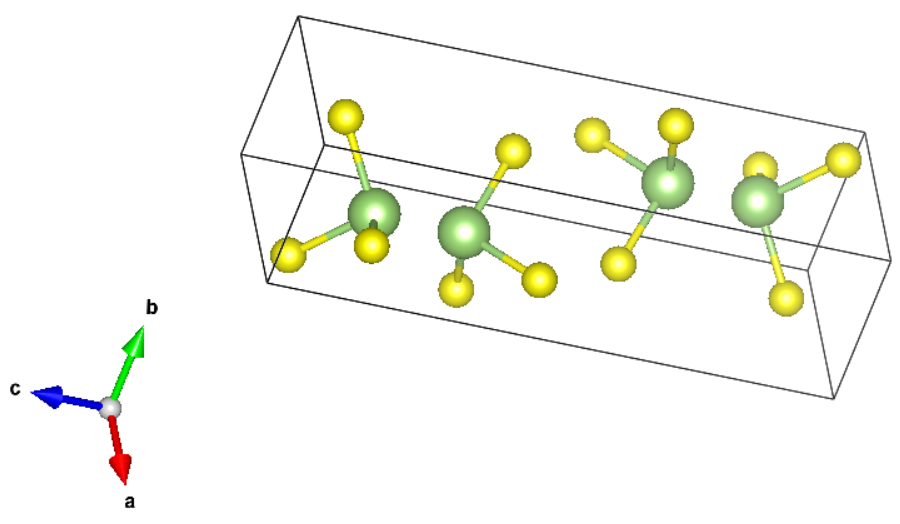
\includegraphics[width=0.85\linewidth]{Wlasciwosci/GaS/GaS_vesta.png}
		\caption{Schematyczne przedstawienie struktury krystalicznej $\mathbf{GaS}$. Przygotowano używając oprogramowania VESTA [5].}
	\end{center}
\end{figure}

W kryształach $\mathbf{GaS}$ dominują słabe siły van der Waalsa w oddziaływaniach międzywarstwowych. Silne wiązania kowalencyjne siły występują pomiędzy atomami wewnątrz warstw.
$\mathbf{GaS}$ jest zaliczany do półprzewodnik szerokopasmowych, o dużym potencjale aplikacyjnym. Oprócz skośnej przerwy energetycznej wynoszącej około $2.5eV$, posiada on nie wiele większą prostą przerwę energetyczną ($2.95eV$). Stąd materiał ten może być wykorzystany do wytworzenia emiterów w zakresie światła niebieskiego [1].

$\mathbf{Ga_{2}S_{3}}$ posiada zupełnie odmienną budowę krystaliczną. Niedopasowanie walencyjne atomów $\mathbf{Ga}$ – III i $\mathbf{S}$ - VI skutkuję dużą ilością uporządkowanych luk galowych. Jedna trzecia miejsc kationowych, czyli pozycji galowych nie jest zajęta. Występujące luki kationowe, w sposób znaczący wpływają na właściwości fizyczne tego materiału i na obszar jego zastosowań. $\mathbf{Ga_{2}S_{3}}$ może krystalizować w następujących fazach: jednoskośna, heksagonalna, kubiczna.

\begin{enumerate}
	\item[\textbf{I}] \textit{Faza $\alpha'$-$\mathbf{Ga_{2}S_{3}}$} \\
	Najbardziej stabilną fazą związku $\mathbf{Ga_{2}S_{3}}$ jest faza $\alpha'$-$\mathbf{Ga_{2}S_{3}}$.
	\begin{itemize}
		\item Ma jednoskośny układ krystalograficzny;
		\item Faza $\alpha'$-$\mathbf{Ga_{2}S_{3}}$ ma prostą przerwę energetyczną o wartości 3.05 - 3.30 eV \footnote{W zależności od źródła.} i skośną przerwę energetyczną o wartości 3.4 eV.
		\item Wytworzone kryształki są jasnożółte lub przezroczyste. Powodem występowania żółtego koloru w tym półprzewodniku, gdzie przerwa energetyczna ma energię większą niż najbardziej energetyczny foton światła widzialnego, jest obecność luk kationowych. Luki te są zlokalizowane w obszarze przerwy zabronionej na poziomie 0.8 - 0.9 eV powyżej od wierzchołka pasma walencyjnego. Te luki tworzą pułapki elektronowe. Elektrony które przechodzą z pasma przewodnictwa do tych pułapek emitują fotony o energii 2.15 - 2.25 eV co odpowiada światłu żółtemu.
		\item Faza ta posiada dwa politypy należące do różnych grup przestrzennych. Parametry komórki elementarnej dla tej fazy w zależności od grupy przestrzennej wynoszą:
		\begin{itemize}
			\item Grupa przestrzenna $Cc$: $a=1.111\;nm$, $b=0.640\;nm$, $c=0.702\;nm$, $\beta=121.17^{\circ}$;
			\item Grupa przestrzenna $Bb$: $a=1.109\;nm$, $b=0.958\;nm$, $c=0.640\;nm$, $\beta=141.15^{\circ}$;
		\end{itemize}
	\end{itemize} 
	
	\begin{figure}[H]
		\begin{center}
			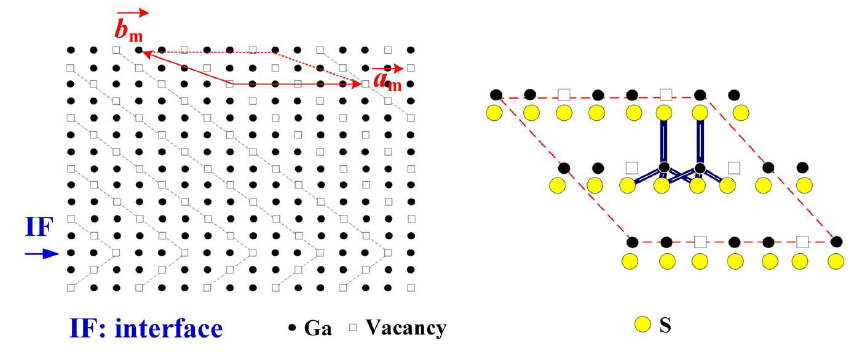
\includegraphics[width=1.0\linewidth]{Wlasciwosci/Przekroj_Ga2S3.png}
			\caption{Na lewym rysunku przedstawiono zdefektowaną sieć krystaliczną w płaszczyźnie prostopadłej do osi c dla związku $\alpha'$-$\mathbf{Ga_{2}S_{3}}$. Luki kationowe (puste kwadraty) tworzą interfejsy w obszarze $\mathbf{Ga_{2}S_{3}}$. Na prawym rysunku pokazano sposób ułożenia i wiązania atomów. Cztery aniony $\mathbf{S}$ w wierzchołkach czworościanu i w środku jeden kation $\mathbf{Ga}$ lub luka.[6]}
		\end{center}
	\end{figure}
	
	\begin{figure}[H]
		\begin{minipage}[h]{0.47\linewidth}
			\center{\includegraphics[width=1\linewidth]{Wlasciwosci/Ga2S3/Cc/Ga2S3_a.png}} a) \\
		\end{minipage}
		\hfill
		\begin{minipage}[h]{0.47\linewidth}
			\center{\includegraphics[width=1\linewidth]{Wlasciwosci/Ga2S3/Cc/Ga2S3_b.png}} \\b)
		\end{minipage}
		\vfill
		\begin{minipage}[h]{0.47\linewidth}
			\center{\includegraphics[width=1\linewidth]{Wlasciwosci/Ga2S3/Cc/Ga2S3_c.png}} c) \\
		\end{minipage}q
		\hfill
		\begin{minipage}[h]{0.47\linewidth}
			\center{\includegraphics[width=1\linewidth]{Wlasciwosci/Ga2S3/Cc/Ga2S3_vesta.png}} d) \\
		\end{minipage}
		\caption{Komórka elementarna dla $\alpha'$-$\mathbf{Ga_{2}S_{3}}$. Grupa przestrzenna $Cc$. Oznaczenia a, b, c, d dotyczą różnych kierunków obserwacji. Przygotowano używając oprogramowanie VESTA.[5]}
		\begin{minipage}[h]{0.47\linewidth}
			\center{\includegraphics[width=1\linewidth]{Wlasciwosci/Ga2S3/Bb/Ga2S3_a.png}} a) \\
		\end{minipage}
		\hfill
		\begin{minipage}[h]{0.47\linewidth}
			\center{\includegraphics[width=1\linewidth]{Wlasciwosci/Ga2S3/Bb/Ga2S3_b.png}} \\b)
		\end{minipage}
		\vfill
		\begin{minipage}[h]{0.47\linewidth}
			\center{\includegraphics[width=1\linewidth]{Wlasciwosci/Ga2S3/Bb/Ga2S3_c.png}} c) \\
		\end{minipage}
		\hfill
		\begin{minipage}[h]{0.47\linewidth}
			\center{\includegraphics[width=1\linewidth]{Wlasciwosci/Ga2S3/Bb/Ga2S3_vesta.png}} d) \\
		\end{minipage}
		\caption{Komórka elementarna dla $\alpha'$-$\mathbf{Ga_{2}S_{3}}$. Grupa przestrzenna $Bb$. Przygotowano używając oprogramowanie VESTA [5].}
	\end{figure}
	
	\item[\textbf{II}] Fazy $\alpha$-$\mathbf{Ga_{2}S_{3}}$ ma grupę przestrzenną $P6_1$. Ta faza ma sześciokątny układ krystalograficzny. Parametry komórki elementarnej $a=0.639\;nm$, $c=1.804\;nm$.
	
	\begin{figure}[H]
		\begin{minipage}[h]{0.47\linewidth}
			\center{\includegraphics[width=1\linewidth]{Wlasciwosci/Ga2S3/alfa/Ga2S3_a.png}} a) \\
		\end{minipage}
		\hfill
		\begin{minipage}[h]{0.47\linewidth}
			\center{\includegraphics[width=1\linewidth]{Wlasciwosci/Ga2S3/alfa/Ga2S3_b.png}} \\b)
		\end{minipage}
		\vfill
		\begin{minipage}[h]{0.47\linewidth}
			\center{\includegraphics[width=1\linewidth]{Wlasciwosci/Ga2S3/alfa/Ga2S3_c.png}} c) \\
		\end{minipage}q
		\hfill
		\begin{minipage}[h]{0.47\linewidth}
			\center{\includegraphics[width=1\linewidth]{Wlasciwosci/Ga2S3/alfa/Ga2S3_vesta.png}} d) \\
		\end{minipage}
		\caption{Komórka elementarna dla $\alpha$-$\mathbf{Ga_{2}S_{3}}$. Przygotowano używając oprogramowanie VESTA [5].}
	\end{figure}

	\item[\textbf{III}] \textit{Faza $\beta$-$\mathbf{Ga_{2}S_{3}}$} \\
	Ta faza jest nazywana fazą $\beta$, z sześciokątnym układem krystalograficznym. Grupa przestrzenna $P6_{3}mc$ Parametry komórki elementarnej: $a=0.368\;nm$,  $c=0.602\;nm$. Faza $\beta$ związku $\mathbf{Ga_{2}S_{3}}$ ma najmniejszą przerwę energetyczną dla tego materiału 2.48 eV.
	
	\begin{figure}[H]
		\begin{minipage}[h]{0.47\linewidth}
			\center{\includegraphics[width=1\linewidth]{Wlasciwosci/Ga2S3/beta/Ga2S3_a.png}} a) \\
		\end{minipage}
		\hfill
		\begin{minipage}[h]{0.47\linewidth}
			\center{\includegraphics[width=1\linewidth]{Wlasciwosci/Ga2S3/beta/Ga2S3_b.png}} \\b)
		\end{minipage}
		\vfill
		\begin{minipage}[h]{0.47\linewidth}
			\center{\includegraphics[width=1\linewidth]{Wlasciwosci/Ga2S3/beta/Ga2S3_c.png}} c) \\
		\end{minipage}q
		\hfill
		\begin{minipage}[h]{0.47\linewidth}
			\center{\includegraphics[width=1\linewidth]{Wlasciwosci/Ga2S3/beta/Ga2S3_vesta.png}} d) \\
		\end{minipage}
		\caption{$\beta$-$\mathbf{Ga_{2}S_{3}}$. Przygotowano używając oprogramowanie VESTA [5].}
	\end{figure}

	\item[\textbf{IV}] \textit{Faza $\gamma$-$\mathbf{Ga_{2}S_{3}}$} \\
	Faza z grupą przestrzenna $F-43m$. Jest to faza niskotemperaturowa. Kryształki $\gamma$-$\mathbf{Ga_{2}S_{3}}$ są białego koloru. Przerwa energetyczna wynosi 2.96 eV. Parametry komórki elementarnej: $a=0.517\;nm$.
	\begin{center}
		\begin{figure}[H]
			\begin{minipage}[h]{0.47\linewidth}
				\center{\includegraphics[width=0.8\linewidth]{Wlasciwosci/Ga2S3/gamma/Ga2S3_vesta.png}} a) \\
			\end{minipage}
			\hfill
			\begin{minipage}[h]{0.47\linewidth}
				\center{\includegraphics[width=0.8\linewidth]{Wlasciwosci/Ga2S3/gamma/Ga2S3_a.png}} \\b)
			\end{minipage}
			\caption{Komórka elementarna dla $\gamma$-$\mathbf{Ga_{2}S_{3}}$. Przygotowano używając oprogramowanie VESTA.[5]}
		\end{figure}
	\end{center}
	
\end{enumerate}

Poniżej została przedstawiona tabela, w której zostały zebrane informację o czterech fazach krystalicznych materiału $\mathbf{Ga_{2}S_{3}}$:
\begin{table}[H]
	\begin{tabular}{|c|c|c|c|c|}
		\hline
		\multicolumn{1}{|l|}{\textbf{Nazwa}} & \textbf{\begin{tabular}[c]{@{}c@{}}Układ \\ krystalograficzny\end{tabular}} & \textbf{\begin{tabular}[c]{@{}c@{}}Grupa\\ przestrzenna\end{tabular}} & \textbf{Typ struktury}                                            & \textbf{\begin{tabular}[c]{@{}c@{}}Parametry sieci\\ krystalicznej\end{tabular}} \\ \hline
		$\alpha$-$\mathbf{Ga_{2}S_{3}}$                              & Heksagonalny                                                               & $P6_{1}$                       & \begin{tabular}[c]{@{}c@{}}Superstruktura \\ wurcytu\end{tabular} & $a=0.639\;nm$,$c=1.804\;nm$                                                                   \\ \hline
		\multirow{2}{*}{$\alpha'$-$\mathbf{Ga_{2}S_{3}}$}            & \multirow{2}{*}{Jednoskośny}                                                & $Cc$                          & \begin{tabular}[c]{@{}c@{}}Superstruktura\\ $\alpha$-$\mathbf{Ga_{2}S_{3}}$\end{tabular}  & 
		\begin{tabular}[c]{@{}c@{}}$a=1.111\;nm$, $b=0.640\;nm$,\\ $c=0.702\;nm$,$\beta=121.17^{\circ}$\end{tabular}                                                                            \\ \cline{3-5} 
		&                                                                             & $Bb$                          & \begin{tabular}[c]{@{}c@{}}Superstruktura\\ $\alpha$-$\mathbf{Ga_{2}S_{3}}$\end{tabular}  & 	
		\begin{tabular}[c]{@{}c@{}}$a=1.109\;nm$, $b=0.958\;nm$,\\ $c=0.640\;nm$, $\beta=141.15^{\circ}$\end{tabular}                                                                            \\ \hline
		$\beta$-$\mathbf{Ga_{2}S_{3}}$                              & Sześciokątny                                                                & $P6_{3}mc$                     & Wurcyt                                                            & $a=0.368\;nm$,                                                                                           $c=0.602\;nm$                                                                              \\ \hline
		$\gamma$-$\mathbf{Ga_{2}S_{3}}$                              & Sześcienny                                                                  & $F$-$43m$                       & Blenda cynkowa                                                    & $a=0.517\;nm$                                                                            \\ \hline
	\end{tabular}
	\caption{Wszystkie fazy krystaliczne $\mathbf{Ga_{2}S_{3}}$.[27]}
\end{table}

Główne piki w widmie rentgenowskim dla każdej z faz $\mathbf{Ga_{2}S_{3}}$ występują praktycznie dla tych samych kątów, jedynie intensywności względne są różne. To oznacza że jeżeli faza kubiczna $\gamma$-$\mathbf{Ga_{2}S_{3}}$ ma strukturę blendy cynkowej $\mathbf{ZnS}$ ze zdefektowaną podsiecią kationową, to i każda z faz też będzie miała zdefektowaną podsieć kationową.

Widma ramanowskie i widma rentgenowskie są prawie takie same dla każdej z faz $\mathbf{Ga_{2}S_{3}}$. Dlatego informacje o strukturze tego materiału w literaturze są niejednoznaczne i często niespójne. Widmo polaryzacyjne dla tego materiału może być bardzo użyteczne dla określenia fazy $\mathbf{Ga_{2}S_{3}}$. W tej pracy zajmuję się badaniem widma polaryzacyjnego dla $\alpha'$-$\mathbf{Ga_{2}S_{3}}$ która ma grupę przestrzenną $Cc$.

Dla wszystkich rysunków, które zostały zrobione za pomocą oprogramowania VESTA, punktem wejściowym są pliki ($\mathbf{CIF}$\footnote{Crystallographic information file (CIF) -- standardowy format pliku tekstowego, służący do zapisu danych krystalograficznych.}).

Poniżej znajduje się zawartość przykładowego pliku ($\mathbf{CIF}$) dla $\alpha'$-$\mathbf{Ga_{2}S_{3}}$:
\begin{lstlisting}
	data_409550-ICSD
	#@2015 by Fachinformationszentrum Karlsruhe, and the U.S. Secretary of 
	#Commerce on behalf of the United States.  All rights reserved.
	_database_code_ICSD                409550
	_audit_creation_date               2002/10/01
	_audit_update_record               2005/04/01
	_chemical_name_systematic          'Digallium Sulfide'
	_chemical_formula_structural       'Ga2 S3'
	_chemical_formula_sum              'Ga2 S3'
	_publ_section_title
	;
	Refinement of the crystal structure of digallium trisulfide, Ga2 S3
	;
	loop_
	_citation_id
	_citation_journal_abbrev
	_citation_year
	_citation_journal_volume
	_citation_page_first
	_citation_page_last
	_citation_journal_id_ASTM
	primary 'Zeitschrift fuer Kristallographie - New Crystal Structures'
	2001 216 327 328 ZKNSFT
	_publ_author_name
	;
	Jones, C.Y.;Bryan, J.C.;Kirschbaum, K.;Edwards, J.G.
	;
	_cell_length_a                     11.107(2)
	_cell_length_b                     6.395(1)
	_cell_length_c                     7.021(1)
	_cell_angle_alpha                  90.
	_cell_angle_beta                   121.17(3)
	_cell_angle_gamma                  90.
	_cell_volume                       426.7
	_cell_formula_units_Z              4
	_symmetry_space_group_name_H-M     'C 1 c 1'
	_symmetry_Int_Tables_number        9
	_refine_ls_R_factor_all            0.035
	loop_
	_symmetry_equiv_pos_site_id
	_symmetry_equiv_pos_as_xyz
	1	'x, -y, z+1/2'
	2	'x, y, z'
	3	'x+1/2, -y+1/2, z+1/2'
	4	'x+1/2, y+1/2, z'
	loop_
	_atom_type_symbol
	_atom_type_oxidation_number
	Ga3+	3
	S2-	-2
	loop_
	_atom_site_label
	_atom_site_type_symbol
	_atom_site_symmetry_multiplicity
	_atom_site_Wyckoff_symbol
	_atom_site_fract_x
	_atom_site_fract_y
	_atom_site_fract_z
	_atom_site_occupancy
	_atom_site_attached_hydrogens
	Ga1 Ga3+ 4 a 0.04213(8) 0.40234(19) 0.12512(11) 1. 0 
	Ga2 Ga3+ 4 a 0.20026(9) 0.93206(18) 0.11559(13) 1. 0 
	S1 S2- 4 a -.0050(3) 1.0861(4) -.0162(6) 1. 0 
	S2 S2- 4 a 0.3378(3) 0.9075(3) 0.4999(4) 1. 0 
	S3 S2- 4 a 0.1741(3) 0.5840(3) 0.0084(4) 1. 0 
	
	loop_
	_atom_site_aniso_label
	_atom_site_aniso_type_symbol
	_atom_site_aniso_U_11
	_atom_site_aniso_U_22
	_atom_site_aniso_U_33
	_atom_site_aniso_U_12
	_atom_site_aniso_U_13
	_atom_site_aniso_U_23
	Ga1 Ga3+ 0.0068(7) 0.0130(6) 0.0096(7) 0.0007(4) 0.0042(5) 0.0005(4)
	Ga2 Ga3+ 0.0065(7) 0.0133(6) 0.0102(7) -.0003(4) 0.0045(5) -.0012(4)
	S1 S2- 0.0065(12) 0.0160(13) 0.0182(13) -.0001(8) 0.0043(10) -.0048(9)
	S2 S2- 0.0041(12) 0.0153(12) 0.0098(15) -.0009(8) 0.0036(11) -.0019(8)
	S3 S2- 0.0084(13) 0.0121(12) 0.0095(12) -.0017(8) 0.0056(10) -.0010(8)
	#End of data_409550-ICSD
\end{lstlisting}
Pliki cif są generowane podczas badań strukturalnych rentgenowskich materiału. Następnie są katalogowane w bazach krystalograficznych. Pliki te są punktem wyjściowym do wygenerowanych w ramach te pracy struktur $\mathbf{Ga_{2}S_{3}}$ przy użyciu programu VESTA. Zawartością tego pliku jest:
\begin{itemize}
	\item Informację ogólne o związku;
	\item Miejsce skąd wzięte te informacje;
	\item Parametry komórki elementarnej;
	\item Grupa symetrii;
	\item Położenia atomów w komórce elementarnej. 
\end{itemize} 

\subsection{Własności i zastosowania $\mathbf{Ga_{2}S_{3}}$}
Jednym z najważniejszych problemów materiałów półprzewodnikowych stosowanych w fotoelektronice jest opracowanie związków o stabilnych właściwościach pod wpływem promieniowania UV, promieniowania rentgenowskiego i $\gamma$, a także opracowanie detektorów promieniowania jonizującego w oparciu o te materiały. Strukturalne defekty w materiale wywoływane są pod wpływem promieni UV, promieniowania rentgenowskiego i $\gamma$. Koncentracja i rodzaj tych defektów zależy zarówno od dawki promieniowania, jak i rodzaju materiału. Detektory promieniowania rentgenowskiego i promieniowania UV oparte na tych materiałach muszą spełniać warunek, że koncentracja ich własnych defektów jest znacznie wyższa niż koncentracja defektów wywołanych promieniowaniem. Materiały takie jak $\mathbf{A_{2}^{III}C_{3}^{VI}}$, szczególnie $\mathbf{Ga_{2}S_{3}}$, spełniają to wymaganie. $\frac{1}{3}$ pozycji w podsieci kationowej są nieobsadzone i tworzą luki, czyli defekty kryształu. Koncentracja własnych defektów w tych materiałach wynosi około $10^{22}\;cm^{-3}$. Przewodność elektryczna pojedynczych kryształów $\mathbf{Ga_{2}S_{3}}$ w normalnej temperaturze wynosi około $10^{-12}\;\Omega^{-1}cm^{-1}$. Przewodność elektryczna wzrasta 3 razy z domieszką $\mathbf{Cd}$.[10][15][28]
\subsubsection{Własności}
\begin{enumerate}
	\item Szerokopasmowa światłoczułość w zakresie blue - UV. Takie promieniowanie elektromagnetyczne trafiając na materiał $\mathbf{Ga_{2}S_{3}}$ zmienia jego przewodność elektryczną. Domieszkując ten materiał można wpływać na światłoczułość;
	\item Fotoluminescencja w zakresie $"$green-blue$"$, to odpowiada przedziału energetycznemu 1.60 - 3.00 eV;
	\item Optyczna nieliniowość. $\mathbf{Ga_{2}S_{3}}$ można wykorzystać do generacji drugiej harmonicznej. Z generacją drugiej harmonicznej mamy do czynienie wówczas gdy na materiał zostanie skierowane promieniowanie o dużej intensywności i monochromatyczności o częstotliwości $\omega$, to obok promieniowania wychodzącego z tego materiału pojawi się również promieniowanie o częstości $2\omega$.
	\item Wysoka przezroczystość w IR. Czyli materiał nie tłumi promieniowania w podczerwieni.
	\item "High damage treshold". Czyli ma dużą odporność na uszkodzenia.
\end{enumerate}

\subsubsection{Zastosowania}

$\mathbf{GaS}$ był przez długi czas uważany jako odpowiedni materiał do aplikacji terahertzowych (THz). Ma bardzo szerokie okna dla promieniowania o długości fali 0.62 – 20 $\mu m$ oraz powyżej 50 $\mu m$. Ale jego warstwowa struktura i wynikające z tego słabe właściwości mechaniczne ograniczają możliwości zastosowania tego materiału. $\mathbf{Ga_{2}S_{3}}$ jest przezroczysty dla fal w zakresie 0.44 – 25 $\mu m$ co jest pokazane na rysunku poniżej. Z tego względu jest obiecującym materiałem na elementy optyczne w zakresie podczerwieni. Wykazuje on również dużą przezroczystość w obszarze terahertzowym. 

\begin{figure}[H]
	\begin{center}
		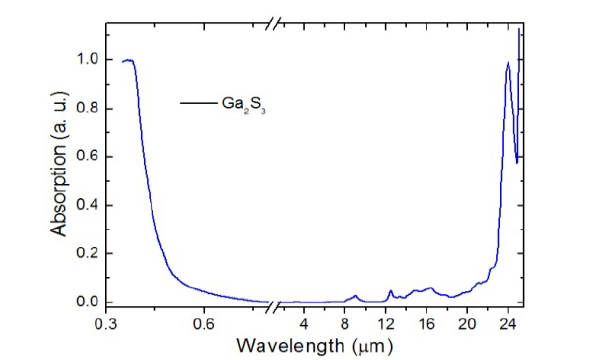
\includegraphics[width=0.8\linewidth]{Wlasciwosci/Widmo-absorpcji-Ga2S3.png}
		\caption{Widmo absorpcji dla $Ga_{2}S_{3}$.[25]}
	\end{center}
\end{figure}

\begin{enumerate}
	\item Materiał $\mathbf{Ga_{2}S_{3}}$ ma zastosowanie optyczne i optoelektroniczne (diody elektroluminescencyjne (LED), absorber UV w fotowoltaicznych urządzeniach, generator drugiej harmonicznej, generator trzeciej harmonicznej np. w materiale $\mathbf{Ti_{2}S}$-$\mathbf{Ga_{2}S_{3}}$-$\mathbf{GeS_{2}}$), ze względu na swoją skośną i szeroką przerwę energetyczną). Struktura cienkowarstwowa Ga2S3/In/Ga2S3 ma potencjalne zastosowanie jako rezonator mikrofalowy. Jego dwójłomność 0,025 jest większa niż $\mathbf{CdSe}$, która pozwala dopasować fazę SHG dla długości fali dłuższej niż 1910 $\mu m$ [22]][26].
	
	\item Kolejne z możliwych zastosowań tego materiału jest pasywacja powierzchni półprzewodnikowej III - V tj. do utworzenia izolującej warstwy siarczkowej na $\mathbf{GaAs}$ lub $\mathbf{InP}$ poprzez siarkowanie na powierzchni; tak, że rekombinacja powierzchni. Dodatkową zaletą tego procesu pasywacji jest zmniejszenie rekombinacji na powierzchni $\mathbf{GaAs}$ lub $\mathbf{InP}$, co z kolei znacząco poprawia wydajność urządzeń na bazie tych materiałów. W dziedzinie nauki o materiałach i technologii brakuje skutecznych warstw pasywacji powierzchniowej  dla $\mathbf{GaAs}$ [30][33]. Należy podkreślić że pasywacja powierzchniowa $\mathbf{GaAs}$ jest procesem bardzo skomplikowanym i generalnie brakuje odpowiednich materiałów dla tego procesu.
	
	\item Materiały $\mathbf{GaS}$ i $\mathbf{Ga_{2}S_{3}}$ mają odpowiednie właściwości do zastosowań w zakresie wzmacniaczy w paśmie telekomunikacyjnym i jako materiały do elementów laserowych [20][29].
	
	\item Dodatkową zaletą tych materiałów jest nietoksyczność i stosunkowo duża odporność mechaniczna i chemiczna.
\end{enumerate}

\subsection{Widmo ramanowskie $\mathbf{Ga_{2}S_{3}}$}

Widmo ramanowskie dla związku $\alpha$-$\mathbf{Ga_{2}S_{3}}$ ma 7 pików, które odpowiadają przesunięciom: 1) 119, 2) 135, 3) 148, 4) 238, 5) 309, 6) 331, 7) 392 $cm^{-1}$.

W budowie krystalicznej $\mathbf{Ga_{2}S_{3}}$ występują tetraedry $[\mathbf{GaS_{4}}]$ co skutkuje tym, że widmo ramanowskie $\mathbf{Ga_{2}S_{3}}$ można podzielić na mody wewnętrzne tetraedru $[\mathbf{GaS_{4}}]$ oraz mody związane
z oddziaływaniami zewnętrznymi.


\begin{figure}[H]
	\begin{center}
		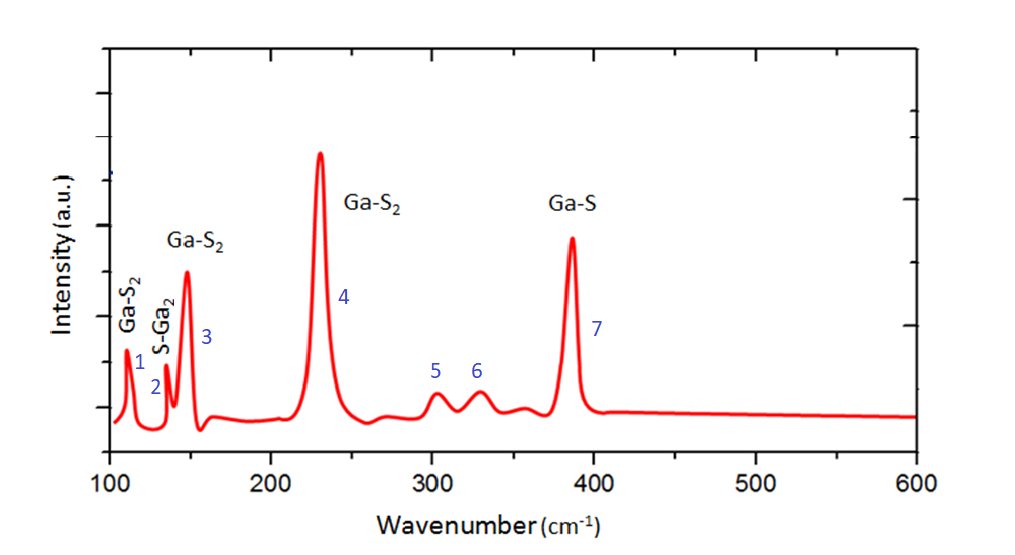
\includegraphics[width=1.0\linewidth]{Wlasciwosci/Raman-Ga2S3.png}
		\caption{Widmo ramanowskie dla $\alpha'$-$\mathbf{Ga_{2}S_{3}}$.[11]}
	\end{center}
\end{figure}

Piki ramanowskie w przedziale 200-450 $cm^{-1}$ są przypisywane drganiom rozciągającym $\mathbf{Ga}$-$\mathbf{S}$. W tym zakresie znajdują się mody A1 i F2. Piki ramanowskie występujące poniżej 200 $cm^{-1}$ są związane z drganiami zginającymi dla tetraedrów $[\mathbf{GaS_{4}}]$. 
W tym zakresie spektralnym występują mody o symetrii E i E2. W zakresie niskich częstości występują również mody translacyjne i rotacyjne dla grup $[\mathbf{GaS_{4}}]$, ale nie są one aktywne ramanowsko. Najbardziej intensywny pik ramanowski dla struktur krystalicznych $\mathbf{Ga_{2}S_{3}}$ jest obserwowany dla około 235 $cm^{-1}$ – jest to mod A1, który jest związany z drganiami siarki w kierunku wakansji galowej. 



